\section{Statistics}
Statistics are obtained by observing the RRD database.  We have tracked both requests and connections made to the server in order to track whether it accomplish the SLA in efficiency terms.
\subsection{General statistics during Operation Phase}
\begin{tabular}{ c c c c }
Server & accepts & handled & requests \\
60884 &  & 60844 & 71613 \\
\end{tabular} \\
Server accepts handled requests: Nginx server accepted 60844 connections.
Handled: 60844 connections (we can see that no one was closed just it was accepted).
Request Handled: 71613 requests (1.17 requests per connection)
\subsection{Monthly Statistics}
These are the number of connections made during this month.  Operation phase corresponds to from 13th week to 16th week. The description of each series is as follows:
\begin{lstlisting}
Reading -- nginx reads request header
Writing -- nginx reads request body, processes request, or writes response to a client
Waiting -- keep-alive connections, actually it is active - (reading + writing)
\end{lstlisting}
We can see a continuous state in the server which means that it had no errors and also that most of operations are responses to clients. Keep-alive connections show us that connections are kept in a short period of time.
Since there is more activity during last week, we show its statisctics.
Statistics are obtained by observing the RRD database.  We have tracked both requests and connections made to the server in order to track whether it accomplish the SLA in efficiency terms.
\subsection{Connection and processed requests reports}
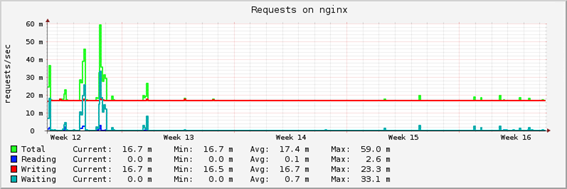
\includegraphics{statistics/img1.png}
These are the number of connections made during this month.  Operation phase corresponds to from 15th week to 16th week. The description of each series is as follows:
\begin{lstlisting}
Reading -- nginx reads request header
Writing -- nginx reads request body, processes request, or writes response to a client
Waiting -- keep-alive connections, actually it is active - (reading + writing)
\end{lstlisting}
We can see a continuous state in the server which means that it had no errors and also that most of operations are responses to clients. Keep-alive connections show us that connections are kept in a short period of time.
Since there is more activity during last week (operation period), we show its statisctics concerning both connections and requests made to the server:\\
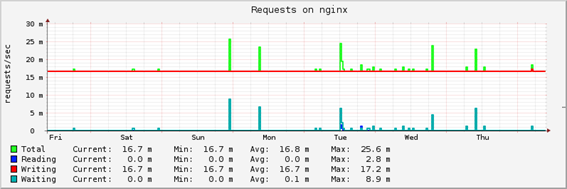
\includegraphics{statistics/img2.png}
 During this week, the requests activity between clients and server was as follows:
\subsection{Requests statistics}
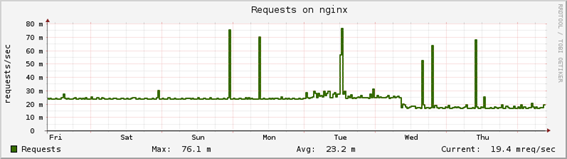
\includegraphics{statistics/img3.png} \\
This graphic shows that the maximum grade of activity in the server was a total of  76.1 mreq/sec. This also shows that the server answered correctly to all requests since there are no holes in the database (the server has not been collapsed).
\pagebreak